\documentclass{beamer}

\usepackage[utf8x]{inputenc}
\usepackage[brazil,english,portuguese]{babel}

\usepackage{graphicx,wrapfig}

\usetheme{Warsaw}

%\usecolortheme{crane}
\usecolortheme{owl}

\setbeamertemplate{background canvas}[vertical shading][bottom=darkgray,top=black]
\setbeamerfont{alerted text}{series=\bfseries} %make alerted text bold
\setbeamercolor{alerted text}{fg=blue} %change the font color
\setbeamertemplate{footline}[frame number]%numerar página

%%% capa
\setbeamerfont{author}{size=\scriptsize,series=\bfseries,parent=structure}
\setbeamerfont{date}{size=\scriptsize,series=\bfseries,parent=structure}

\title[Enhancing Moodle with External Data Integration]{Enhancing Moodle with External Data Integration:\\A Case Study at the University of São Paulo}
\author{Thiago Gomes Veríssimo \\ Ewout ter Haar \\ Paulo Roberto Miranda Meirelles}
\institute{University of São Paulo}
\date{19 June 2024}

% logo of my university
\titlegraphic{
    \small Learning Analytics in Practice 2024
    
\includegraphics[width=2cm]{../../images/logo_usp_branco.png}\hspace*{4.75cm}~%
    
\includegraphics[width=2cm]{../../images/lap24.png}
}

\begin{document}

\begin{frame}
\titlepage
\end{frame}

\begin{frame}{Outline}
    \tableofcontents
\end{frame}

\section{Introduction}

\begin{frame}{Context}
    Our aim is to study, scientifically, the construction of Learning Analytics Dashboards and related software engineering issues.

    \begin{figure}[H]
        \centering
        \label{fig:digital_learning}
        %\caption{The data regarding the student learning process is dispersed across multiple sources} 
        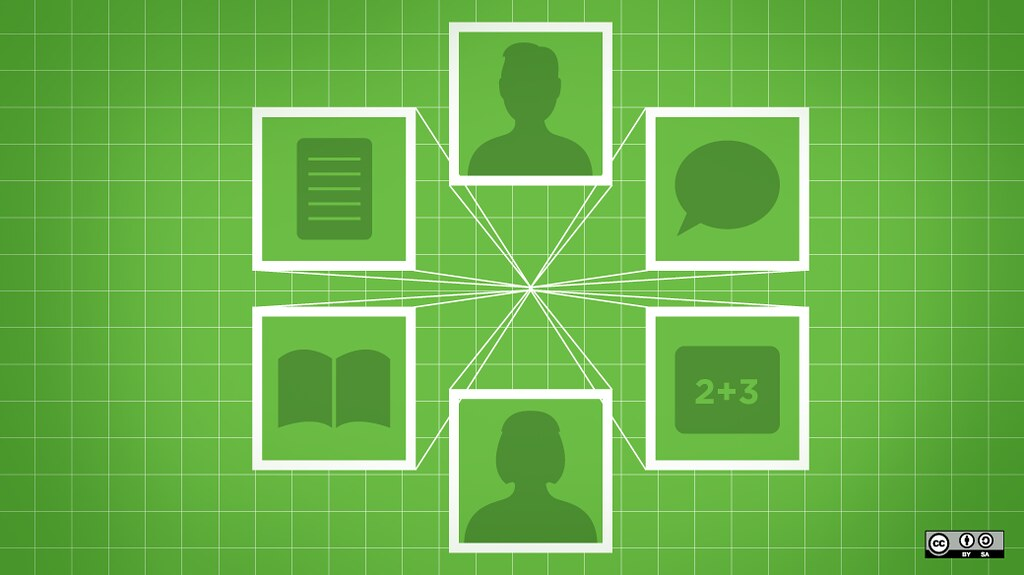
\includegraphics[width=0.5\textwidth]{../../images/digital_learning.jpg}
        \\ \small The data regarding the student learning process is dispersed across multiple sources
        \\ \small \url{https://www.flickr.com/photos/opensourceway/8288335386/}
    \end{figure}

    It is a Learning Analytics research field \cite{lang2017handbook}.
\end{frame}


\begin{frame}{The journey up to this point}
    \begin{figure}[H]
        \centering
        \includegraphics[width=1\textwidth]{../../../thiago-doutorado-ime-usp/outputs/timeline.pdf}
    \end{figure}
\end{frame}

\subsection{Research Questions}
\begin{frame}{Research Questions (temporary yet)}
    \begin{enumerate}[<+-|alert@+>]\color{gray}
        \item What kind of external data can be usefully and safely integrated with 
              the Moodle (behavioral) data?
        \item How this enriched data can be used as features for Statistical and 
              Machine Learning models (to be presented in dashboards) respecting privacy and student autonomy?
    \end{enumerate}
\end{frame}

\begin{frame}{Our proposal}
    The traditional approach used to build dashboards (we are currently confirming through a Systematic Literature Review):

    \begin{table}[]
        \begin{tabular}{|l|l|l|} \hline
                 & Can choose Features? & Can see Predictions?\\ \hline
         Student & No                   & No                  \\ \hline
         Teacher & No                   & Yes                 \\ \hline
         Manager & Yes                  & Yes                 \\ \hline
        \end{tabular}
    \end{table}

    \pause
    Our proposal: Student \underline{in Control} Perspective
    \pause
    \begin{table}[]
        \begin{tabular}{|l|l|l|} \hline
                 & Can choose Features?  & Can see Predictions?                    \\ \hline
         Student & \textcolor{red}{Yes}  & \textcolor{red}{Yes}                    \\ \hline
         Teacher & No                    & \textcolor{blue}{Maybe} (student decides) \\ \hline
         Manager & No                    & \textcolor{blue}{Maybe} (student decides) \\ \hline
        \end{tabular}
    \end{table}

\end{frame}

\begin{frame}{Software Engineering Issues}

    \begin{figure}
        \centering
        \begin{minipage}{.7\textwidth}
            Some issues this approach brings to software engineering:
        \end{minipage}%
        \begin{minipage}{.25\textwidth}
          \centering
          
\includegraphics[width=0.8\textwidth]{../../images/work-workers-men.jpg}
        \end{minipage}
    \end{figure}

    \begin{itemize}[<+-|alert@+>]\color{gray}
        \item The Moodle Analytics API is designed primarily for teachers and managers, so a lot of 
              work is needed on plugins to empower students with similar capabilities
        \item The possibility for each student to choose their own data requires 
              rebuilding the model many times, which can impact performance
    \end{itemize}
\end{frame}


\section{Metodologia}

\begin{frame}{Revisão Terciária}
    Questão de pesquisa formulada para a revisão terciária: 

    \emph{Qual o perfil das revisões sistemáticas existentes com foco em painéis de análise de aprendizagem?}
\end{frame}

\begin{frame}{Revisão Terciária}
  Metodologia de revisão sistemática proposta por \cite{Kitchenham:2007}:
  \begin{itemize}
    \begin{spacing}{0.3}
      \item 1. Planejamento: Definição da Questão de Pesquisa
      \item 2. Planejamento: Desenvolvimento do Protocolo de Revisão
      \item 3. Planejamento: Definição dos critérios de inclusão e de exclusão
      \item 4. Condução Busca Sistemática e Seleção de Estudos
      \item 5. Condução: Extração de Dados
      \item 6. Condução: Síntese e Análise dos Dados
      \item 7. Condução: Avaliação da Qualidade
      \item 8. Resultados: Interpretação dos Resultados
      \item 9. Resultados: Relato dos Resultados
    \end{spacing}
  \end{itemize}
\end{frame}

\begin{frame}{Revisão Terciária}
    \textbf{Cadeia de busca:}

    \textit{"Dashboard" AND "Learning Analytics" AND ("Systematic Literature Review" OR "Systematic Review")}
\end{frame}

\begin{frame}{Revisão Terciária}
    \input{/tmp/tertiary_review_databases_duplicated.tex}
\end{frame}


\begin{frame}{Revisão Terciária}
    {\tiny
    \input{/tmp/tertiary_review_excluded.tex}
    }
\end{frame}

\begin{frame}{Revisão Terciária}
    \begin{figure}[H]
        \centering
        \label{fig:digital_learning}
        %\caption{The data regarding the student learning process is dispersed across multiple sources} 
        \includegraphics[width=0.8\textwidth]{/tmp/tertiary_review_yearly_barplot.pdf}
        \\ \small Quantidade de publicações selecionadas por ano
    \end{figure}
\end{frame}

\begin{frame}{Revisão Terciária}
    {\tiny
    \begin{itemize}
        \begin{spacing}{0.3}
        \item Q1: Quandidade de bases de dados consultadas
        \item Q2: Arcabouço usado na revisão sistemática
        \item Q3: Quantidade de publicações inicialmente selecionadas a partir da cadeia de busca
        \item Q4: Quantidade de publicações resultantes depois de removidos os duplicados 
        \item Q5: Quantidade de publicações resultantes depois de aplicado os critérios de inclusão e exclusão nos títulos e resumos
        \item Q6: Quantidade de artigos finais selecionados da revisão
        \item Q7: Período inical da coleta
        \item Q8: Período final da coleta
        \item Q9: Razão percentual entre Quantidade de artigos finais e Quantidade de publicações inicialmente selecionadas
        \end{spacing}
    \end{itemize}
    }
\end{frame}
  
\begin{frame}{Revisão Terciária}
    {\tiny
        \input{/home/thiago/repos/thiago-doutorado-ime-usp/data/systematic_review/selecionados.tex}
    }
\end{frame}





\section{Discussion}

\begin{frame}{Discussion}

    \begin{figure}
        \centering
        \begin{minipage}{.25\textwidth}
          \centering
          
\includegraphics[width=0.8\textwidth]{../../images/privacy.png}
        \end{minipage}%
        \begin{minipage}{.7\textwidth}
            Storing sensitive student data, as in the previous case, requires careful consideration 
            of data security and privacy (in human rights sense). 
            Some possible issues:
        \end{minipage}
    \end{figure}

    \begin{itemize}[<+-|alert@+>]\color{gray}
        \item Compliance with Regulations: Ensure compliance with data protection regulations, such as GDPR, FERPA, or other relevant laws
        \item Access Control
        \item User Consent, Transparency
        \item Secure Coding Practices
    \end{itemize}
    
\end{frame}

\begin{frame}{Our proposal}
    The traditional approach used to build dashboards (we are currently confirming through a systematic review):

    \begin{table}[]
        \begin{tabular}{|l|l|l|} \hline
                 & Can choose Features? & Can see Predictions?\\ \hline
         Student & No                   & No                  \\ \hline
         Teacher & No                   & Yes                 \\ \hline
         Manager & Yes                  & Yes                 \\ \hline
        \end{tabular}
    \end{table}

    \pause
    Our proposal: Student in Control Perspective
    \pause
    \begin{table}[]
        \begin{tabular}{|l|l|l|} \hline
                 & Can choose Features? & Can see Predictions?    \\ \hline
         Student & \textbf{Yes}         & \textbf{Yes}            \\ \hline
         Teacher & No                   & Maybe (student decides) \\ \hline
         Manager & No                   & No                      \\ \hline
        \end{tabular}
    \end{table}

\end{frame}

\begin{frame}{Software Engineering}

    \begin{figure}
        \centering
        \begin{minipage}{.7\textwidth}
            Some issues this approach brings to software engineering:
        \end{minipage}%
        \begin{minipage}{.25\textwidth}
          \centering
          
\includegraphics[width=0.8\textwidth]{../../images/work-workers-men.jpg}
        \end{minipage}
    \end{figure}

    \begin{itemize}[<+-|alert@+>]\color{gray}
        \item The Moodle Analytics API is designed primarily for teachers and managers, so a lot of 
              work is needed on plugins to empower students with similar capabilities
        \item The possibility for each student to choose their own indicators requires 
              rebuilding the model many times, which can impact performance
    \end{itemize}
\end{frame}


\section{Conclusion}

\begin{frame}{Conclusion}
    This is a work-in-progress project where we propose to place students in the role of 
    decision-makers to gather insights from prediction models. 
    \\
    Moreover, students will decide what data should be included or excluded from the model.
    \\
    This approach involves addressing several software engineering issues.

    \begin{table}[]
        \begin{tabular}{|l|l|l|} \hline
                 & Can choose Features?  & Can see Predictions?                    \\ \hline
         Student & \textcolor{red}{Yes}  & \textcolor{red}{Yes}                    \\ \hline
         Teacher & No                    & \textcolor{blue}{Maybe} (student decides) \\ \hline
         Manager & No                    & \textcolor{blue}{Maybe} (student decides) \\ \hline
        \end{tabular}
    \end{table}
\end{frame}


\begin{frame}{Conclusion}
    \center{\huge Thank you!}
\end{frame}



\begin{frame}{Bibliography}
    \bibliographystyle{apalike2}
    \bibliography{bibliography}
\end{frame}

\end{document}
